\section{Battery State of Charge}
Battery state of charge (SOC) plays a central role in the bus charge
problem. Battery charge levels decay as a bus traverses a
route. Solutions to the bus charge problem must account for bus routes
and require that SOC values remain above a minimum threshold.
\par A SOC thresholding constraint requires that battery charge levels
be modeled. The $k^{\text{th}}$ SOC for bus $i$ is denoted $d_{i,k}$,
where $k$ is the \textit{node index}. The node indices used here are
not directly tied to specific time steps.  For example, $d_{i,k+1}$
represents the bus SOC at the node in the graph following the node
where $d_{i,k}$ is the SOC as seen in figure~\ref{fig:dSocDiagram}. The set of all $d_{i,k}$ can be organized as the vector $\mathbf{d}$ from equation (\ref{eqn:y}).
\par Because no charging is performed while on route, $d_{i,k}$ will
assume its lowest value when buses enter the charge station. Let $d_{i,k+1}$ be the charge level for bus $i$ as it enters the charge station, and $\delta_i$ represent the power discharged while on-route. The entrance SOC can be expressed as 
\begin{align}\label{eqn:dDelta}
	d_{i,k+1} = d_{i,k} - \delta_i,
\end{align}
where $d_{i,k}$ is the previous departure SOC for bus $i$. Consider the example in figure~\ref{fig:graphDelta}, where buses $1$ and $2$ leave the station at $t_2$ and enter at $t_4$. The corresponding change in SOC is given as $d_{1,2} = d_{1,1} - \delta_1$ and $d_{2,2} = d_{2,1} - \delta_2$ for buses $1$ and $2$ respectively.
\begin{figure}
	\centering
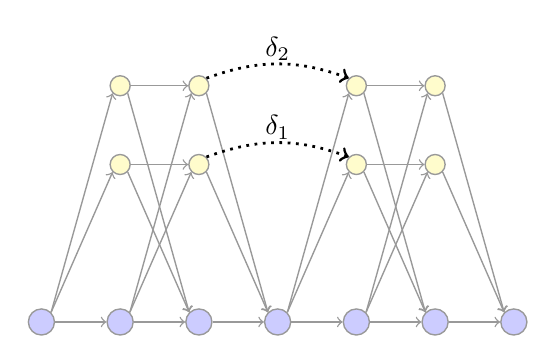
\begin{tikzpicture}
	\node[circle, fill=blue!20, line width=0.5pt, draw=black!40, minimum size=0.1in](one) at (0,0){};
	\node[circle, fill=blue!20, line width=0.5pt, draw=black!40, minimum size=0.1in](two) at (1,0){}; 
	\node[circle, fill=blue!20, line width=0.5pt, draw=black!40, minimum size=0.1in](three) at (2,0){};
	\node[circle, fill=blue!20, line width=0.5pt, draw=black!40, minimum size=0.1in](four) at (3,0){};
	\node[circle, fill=blue!20, line width=0.5pt, draw=black!40, minimum size=0.1in](five) at (4,0){};
	\node[circle, fill=blue!20, line width=0.5pt, draw=black!40, minimum size=0.1in](six) at (5,0){};
	\node[circle, fill=blue!20, line width=0.5pt, draw=black!40, minimum size=0.1in](seven) at (6,0){};
	
	\node[circle, fill=yellow!20, line width=0.5pt, draw=black!40, minimum size=0.1in, inner sep=1pt](eight) at (1,2){};
	\node[circle, fill=yellow!20, line width=0.5pt, draw=black!40, minimum size=0.1in, inner sep=1pt](nine) at (2,2){};
	\node[circle, fill=yellow!20, line width=0.5pt, draw=black!40, minimum size=0.1in, inner sep=1pt](ten) at (4,2){};
	\node[circle, fill=yellow!20, line width=0.5pt, draw=black!40, minimum size=0.1in, inner sep=1pt](eleven) at (5,2){};

	\node[circle, fill=yellow!20, line width=0.5pt, draw=black!40, minimum size=0.1in, inner sep=1pt](twelve) at (1,3){};
	\node[circle, fill=yellow!20, line width=0.5pt, draw=black!40, minimum size=0.1in, inner sep=1pt](thirteen) at (2,3){};
	\node[circle, fill=yellow!20, line width=0.5pt, draw=black!40, minimum size=0.1in, inner sep=1pt](fourteen) at (4,3){};
	\node[circle, fill=yellow!20, line width=0.5pt, draw=black!40, minimum size=0.1in, inner sep=1pt](fifteen) at (5,3){};

	\draw [->, line width=0.5pt, color=black!40] (one.east) -- (two.west);
	\draw [->, line width=0.5pt, color=black!40] (two.east) -- (three.west);
	\draw [->, line width=0.5pt, color=black!40] (three.east) -- (four.west);
	\draw [->, line width=0.5pt, color=black!40] (four.east) -- (five.west);
	\draw [->, line width=0.5pt, color=black!40] (five.east) -- (six.west);
	\draw [->, line width=0.5pt, color=black!40] (six.east) -- (seven.west);

	\draw [->, line width=0.5pt, color=black!40] (one.north east) -- (eight.south west);
	\draw [->, line width=0.5pt, color=black!40] (two.north east) -- (nine.south west);
	\draw [->, line width=0.5pt, color=black!40] (four.north east) -- (ten.south west);
	\draw [->, line width=0.5pt, color=black!40] (five.north east) -- (eleven.south west);
	\draw [->, line width=0.5pt, color=black!40] (eight.south east) -- (three.north west);
	\draw [->, line width=0.5pt, color=black!40] (nine.south east) -- (four.north west);
	\draw [->, line width=0.5pt, color=black!40] (ten.south east) -- (six.north west);
	\draw [->, line width=0.5pt, color=black!40] (eleven.south east) -- (seven.north west);
	\draw [->, line width=0.5pt, color=black!40] (eight.east) -- (nine.west);
	\draw [->, line width=0.5pt, color=black!40] (ten.east) -- (eleven.west); 

	\draw [->, line width=0.5pt, color=black!40] (one.north east) -- (twelve.south west);
	\draw [->, line width=0.5pt, color=black!40] (two.north east) -- (thirteen.south west);
	\draw [->, line width=0.5pt, color=black!40] (four.north east) -- (fourteen.south west);
	\draw [->, line width=0.5pt, color=black!40] (five.north east) -- (fifteen.south west);
	\draw [->, line width=0.5pt, color=black!40] (twelve.south east) -- (three.north west);
	\draw [->, line width=0.5pt, color=black!40] (thirteen.south east) -- (four.north west);
	\draw [->, line width=0.5pt, color=black!40] (fourteen.south east) -- (six.north west);
	\draw [->, line width=0.5pt, color=black!40] (fifteen.south east) -- (seven.north west);
	\draw [->, line width=0.5pt, color=black!40] (twelve.east) -- (thirteen.west);
	\draw [->, line width=0.5pt, color=black!40] (fourteen.east) -- (fifteen.west); 
	\draw [dotted, color=black,-,line width=1pt] (nine.north east) edge[->,bend left=20pt]node[above=-2.5pt]{\scalebox{1}{$\delta_1$}}(ten.north west); 
	\draw [dotted, color=black,-,line width=1pt] (thirteen.north east) edge[->,bend left=20pt]node[above=-2.5pt]{\scalebox{1}{$\delta_2$}}(fourteen.north west); 
\end{tikzpicture}
	\caption{$\delta$ values for routes}
	\label{fig:graphDelta}
\end{figure} 

The constraints from equation (\ref{eqn:dDelta}) can be expressed in linear standard form as 
\begin{equation}\label{eqn:delta2}
	\begin{bmatrix}
		-1 & 1
	\end{bmatrix}
	\begin{bmatrix}
		d_{i,k} \\ d_{i,k+1}
	\end{bmatrix} = \delta_i.
\end{equation}
Equation (\ref{eqn:delta2}) can be expressed in terms of $\mathbf{y}$ with appropriate zero padding and expanded to account for the decrease in SOC for all buses outside the station. The expanded constraint is given as 
\begin{equation}\label{eqn:deltaFinal}
	\begin{aligned}
		\begin{bmatrix}0 & \hdots & -1_{d_{i,k}} & 0 & \hdots & 1_{d_{i,k+1}} \end{bmatrix} \mathbf{y} &= \mathbf{d}_\delta \\
			D_\delta\mathbf{y} &= \mathbf{d}_\delta,
	\end{aligned}
\end{equation}
where $-1_{d_{i,k}}$ and $1_{d_{i,k+1}}$ represent $-1$ and $1$ in locations corresponding to $d_{i,k}$ and $d_{i,k+1}$ respectively. Similar notation will be used throughout this paper as a means to imply a corresponding index for other variables.
\par Time periods between entrance and exit nodes represent time spent in the charge station and have the potential to charge the battery. An edge over which charging occurs is referred to as $x_{i,k}$, where $k$ gives the index of the edge's outgoing node, and $i$ refers to the bus.  When a charger occupies $x_{i,k}$, the resulting increase, or \textit{gain}, in battery charge is denoted $g_{i,k}$, where $i$ and $k$ mirror the edge indices (see figure~\ref{fig:dSocDiagram}). 
\par The value for $g_{i,k}$ is computed using a single charge rate. Multiple charge rates can be encoded by connecting bus nodes with multiple edges, denoted $x_{i,k,l}$, where each edge has a distinct charge rate and gain denoted $g_{i,k,l}$ (see figure~\ref{fig:multirateChargeEdges}). Having multiple charge rates gives the option for fast charging when necessary, and slow charging when possible to preserve battery health and decrease the electrical load \cite{houbbadi_optimal_2019}.
\begin{figure}
	\centering
	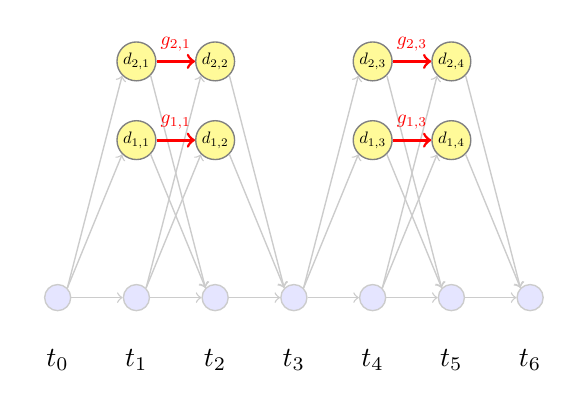
\begin{tikzpicture} 
		\node[circle, fill=blue!10, line width=0.5pt, draw=black!20, minimum size=0.1in](one) at (0,0){};
		\node[circle, fill=blue!10, line width=0.5pt, draw=black!20, minimum size=0.1in](two) at (1,0){}; 
		\node[circle, fill=blue!10, line width=0.5pt, draw=black!20, minimum size=0.1in](three) at (2,0){};
		\node[circle, fill=blue!10, line width=0.5pt, draw=black!20, minimum size=0.1in](four) at (3,0){};
		\node[circle, fill=blue!10, line width=0.5pt, draw=black!20, minimum size=0.1in](five) at (4,0){};
		\node[circle, fill=blue!10, line width=0.5pt, draw=black!20, minimum size=0.1in](six) at (5,0){};
		\node[circle, fill=blue!10, line width=0.5pt, draw=black!20, minimum size=0.1in](seven) at (6,0){};
		
		\node[circle, fill=yellow!40, line width=0.5pt, draw=black!50, minimum size=0.1in, inner sep=1pt](eight) at (1,2){\scalebox{0.6}{$d_{1,1}$}};
		\node[circle, fill=yellow!40, line width=0.5pt, draw=black!50, minimum size=0.1in, inner sep=1pt](nine) at (2,2){\scalebox{0.6}{$d_{1,2}$}};
		\node[circle, fill=yellow!40, line width=0.5pt, draw=black!50, minimum size=0.1in, inner sep=1pt](ten) at (4,2){\scalebox{0.6}{$d_{1,3}$}};
		\node[circle, fill=yellow!40, line width=0.5pt, draw=black!50, minimum size=0.1in, inner sep=1pt](eleven) at (5,2){\scalebox{0.6}{$d_{1,4}$}};

		\node[circle, fill=yellow!40, line width=0.5pt, draw=black!50, minimum size=0.1in, inner sep=1pt](twelve) at (1,3){\scalebox{0.6}{$d_{2,1}$}};
		\node[circle, fill=yellow!40, line width=0.5pt, draw=black!50, minimum size=0.1in, inner sep=1pt](thirteen) at (2,3){\scalebox{0.6}{$d_{2,2}$}};
		\node[circle, fill=yellow!40, line width=0.5pt, draw=black!50, minimum size=0.1in, inner sep=1pt](fourteen) at (4,3){\scalebox{0.6}{$d_{2,3}$}};
		\node[circle, fill=yellow!40, line width=0.5pt, draw=black!50, minimum size=0.1in, inner sep=1pt](fifteen) at (5,3){\scalebox{0.6}{$d_{2,4}$}};

		\draw [->, line width=0.5pt, color=black!20] (one.east) -- (two.west);
		\draw [->, line width=0.5pt, color=black!20] (two.east) -- (three.west);
		\draw [->, line width=0.5pt, color=black!20] (three.east) -- (four.west);
		\draw [->, line width=0.5pt, color=black!20] (four.east) -- (five.west);
		\draw [->, line width=0.5pt, color=black!20] (five.east) -- (six.west);
		\draw [->, line width=0.5pt, color=black!20] (six.east) -- (seven.west);

		\draw [->, line width=0.5pt, color=black!20] (one.north east) -- (eight.south west);
		\draw [->, line width=0.5pt, color=black!20] (two.north east) -- (nine.south west);
		\draw [->, line width=0.5pt, color=black!20] (four.north east) -- (ten.south west);
		\draw [->, line width=0.5pt, color=black!20] (five.north east) -- (eleven.south west);
		\draw [->, line width=0.5pt, color=black!20] (eight.south east) -- (three.north west);
		\draw [->, line width=0.5pt, color=black!20] (nine.south east) -- (four.north west);
		\draw [->, line width=0.5pt, color=black!20] (ten.south east) -- (six.north west);
		\draw [->, line width=0.5pt, color=black!20] (eleven.south east) -- (seven.north west);

		\draw [->, line width=0.5pt, color=black!20] (one.north east) -- (twelve.south west);
		\draw [->, line width=0.5pt, color=black!20] (two.north east) -- (thirteen.south west);
		\draw [->, line width=0.5pt, color=black!20] (four.north east) -- (fourteen.south west);
		\draw [->, line width=0.5pt, color=black!20] (five.north east) -- (fifteen.south west);
		\draw [->, line width=0.5pt, color=black!20] (twelve.south east) -- (three.north west);
		\draw [->, line width=0.5pt, color=black!20] (thirteen.south east) -- (four.north west);
		\draw [->, line width=0.5pt, color=black!20] (fourteen.south east) -- (six.north west);
		\draw [->, line width=0.5pt, color=black!20] (fifteen.south east) -- (seven.north west);
		\draw [->, line width=1pt, color=red] (twelve.east) -- node[above]{\scalebox{0.7}{$g_{2,1}$}}(thirteen.west);
		\draw [->, line width=1pt, color=red] (fourteen.east) -- node[above]{\scalebox{0.7}{$g_{2,3}$}}(fifteen.west); 
		\draw [->, line width=1pt, color=red] (eight.east) -- node[above]{\scalebox{0.7}{$g_{1,1}$}}(nine.west);
		\draw [->, line width=1pt, color=red] (ten.east) -- node[above]{\scalebox{0.7}{$g_{1,3}$}}(eleven.west); 

		\node[rectangle, minimum width=0.3in, minimum height=1.2in,label=below:$t_0$](time0Box) at (0,1){};
		\node[rectangle, minimum width=0.3in, minimum height=1.2in,label=below:$t_1$](time1Box) at (1,1){};
		\node[rectangle, minimum width=0.3in, minimum height=1.2in,label=below:$t_2$](time2Box) at (2,1){};
		\node[rectangle, minimum width=0.3in, minimum height=1.2in,label=below:$t_3$](time3Box) at (3,1){};
		\node[rectangle, minimum width=0.3in, minimum height=1.2in,label=below:$t_4$](time4Box) at (4,1){};
		\node[rectangle, minimum width=0.3in, minimum height=1.2in,label=below:$t_5$](time5Box) at (5,1){};
		\node[rectangle, minimum width=0.3in, minimum height=1.2in,label=below:$t_6$](time6Box) at (6,1){}; 

	\end{tikzpicture}
	\caption{Depiction of which edges increase SOC for the single rate case}
	\label{fig:dSocDiagram}
\end{figure}



\begin{figure}
	\centering
	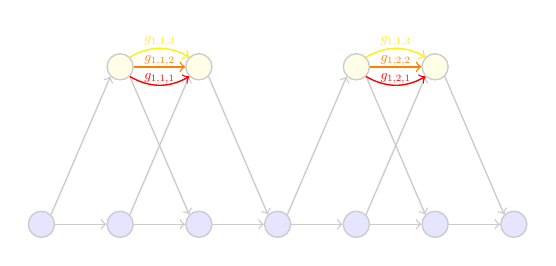
\begin{tikzpicture}[->, line width=0.5pt]
		\node[circle, fill=blue!10, draw=black!20,line width=0.5pt, minimum size=0.1in](one) at (0,0){};
		\node[circle, fill=blue!10, draw=black!20,line width=0.5pt, minimum size=0.1in](two) at (1,0){}; 
		\node[circle, fill=blue!10, draw=black!20,line width=0.5pt, minimum size=0.1in](three) at (2,0){};
		\node[circle, fill=blue!10, draw=black!20,line width=0.5pt, minimum size=0.1in](four) at (3,0){};
		\node[circle, fill=blue!10, draw=black!20,line width=0.5pt, minimum size=0.1in](five) at (4,0){};
		\node[circle, fill=blue!10, draw=black!20,line width=0.5pt, minimum size=0.1in](six) at (5,0){};
		\node[circle, fill=blue!10, draw=black!20,line width=0.5pt, minimum size=0.1in](seven) at (6,0){};
		\node[circle, fill=yellow!10, draw=black!20,line width=0.5pt, minimum size=0.1in](eight) at (1,2){};
		\node[circle, fill=yellow!10, draw=black!20,line width=0.5pt, minimum size=0.1in](nine) at (2,2){};
		\node[circle, fill=yellow!10, draw=black!20,line width=0.5pt, minimum size=0.1in](ten) at (4,2){}; 
		\node[circle, fill=yellow!10, draw=black!20,line width=0.5pt, minimum size=0.1in](eleven) at (5,2){}; 
		\draw [line width=0.5pt,color=black!20] (one.east) -- (two.west);
		\draw [line width=0.5pt,color=black!20] (two.east) -- (three.west);
		\draw [line width=0.5pt,color=black!20] (three.east) -- (four.west);
		\draw [line width=0.5pt,color=black!20] (four.east) -- (five.west);
		\draw [line width=0.5pt,color=black!20] (five.east) -- (six.west);
		\draw [line width=0.5pt,color=black!20] (six.east) -- (seven.west);
		\draw [line width=0.5pt,color=black!20] (one.north east) -- (eight.south west);
		\draw [line width=0.5pt,color=black!20] (two.north east) -- (nine.south west);
		\draw [line width=0.5pt,color=black!20] (four.north east) -- (ten.south west);
		\draw [line width=0.5pt,color=black!20] (five.north east) -- (eleven.south west);
		\draw [line width=0.5pt,color=black!20] (eight.south east) -- (three.north west);
		\draw [line width=0.5pt,color=black!20] (nine.south east) -- (four.north west);
		\draw [line width=0.5pt,color=black!20] (ten.south east) -- (six.north west);
		\draw [line width=0.5pt,color=black!20] (eleven.south east) -- (seven.north west);

		\draw [color=yellow,-,line width=0.5pt] (eight.north east) edge[->,bend left]node[above=-3pt]{\scalebox{0.5}{$g_{1,1,3}$}}(nine.north west);
		\draw [color=orange,line width=0.5pt] (eight.east) -- node[above=-3pt]{\scalebox{0.5}{$g_{1,1,2}$}}(nine.west);
		\draw [color=red,-,line width=0.5pt] (eight.south east) edge[->, bend right]node[above=-3pt]{\scalebox{0.5}{$g_{1,1,1}$}}(nine.south west);

		\draw [color=yellow,-, line width=0.5pt] (ten.north east) edge[->, bend left]node[above=-3pt]{\scalebox{0.5}{$g_{1,1,3}$}}(eleven.north west);
		\draw [color=orange,line width=0.5pt] (ten.east) -- node[above=-3pt]{\scalebox{0.5}{$g_{1,2,2}$}}(eleven.west); 
		\draw [color=red,-, line width=0.5pt] (ten.south east) edge[->, bend right]node[above=-3pt]{\scalebox{0.5}{$g_{1,2,1}$}}(eleven.south west);
	\end{tikzpicture}
	\caption{Multi-Rate Charging}
	\label{fig:multirateChargeEdges}
\end{figure} 

\par The rate is selected by setting $x_{i,k,l} = 1$. All gains associated with unselected rates are set to zero. Gains that correspond to selected rates are computed using the constant current constant voltage (CCCV) model as derived in \cite{whitaker_network_2021} which gives:
\begin{align}\label{eqn:CCCV}
	d_{i,k+1} = \bar{a}_ld_{i,k} - \bar{b}_lM, 
\end{align}
where $\bar{a}_l$ $\sim(0,1]$, depends on the charge rate and is experimentally determined, $M$ is the battery capacity in kWh, and $\bar{b}_l = \bar{a}_l - 1$.
Equation (\ref{eqn:CCCV}) is used to show that
\begin{equation}\label{eqn:g}
\begin{aligned}
	d_{i,k+1} &= \bar{a}_ld_{i,k} - \bar{b}_lM \\ 
	d_{i,k+1} - d_{i,k} &= \bar{a}_ld_{i,k} - \bar{b}_lM - d_{i,k},\\
\end{aligned}
\end{equation}
but the gain is equal to the difference in $d_{i,k+1}$ and $d_{i,k}$ such that $g_{i,k,l} = d_{i,k+1} - d_{i,k}$.  So
\begin{equation}\label{eqn:CCCVFinal}
\begin{aligned}
	g_{i,k,l}  &= \bar{a}_ld_{i,k} - \bar{b}_lM - d_{i,k}\\
	g_{i,k,l}  &= (\bar{a}_l - 1)d_{i,k} - \bar{b_l}M.\\
\end{aligned}
\end{equation}

Therefore, 
\begin{equation}\label{eqn:initialGConstr}
	\begin{aligned}
		\begin{dcases}
			g_{i,k,l} = d_{i,k}(\bar{a}_l - 1) - \bar{b}_lM & x_{i,k,l} = 1\\
			g_{i,k,l} = 0 & x_{i,k,l} = 0
		\end{dcases}.
	\end{aligned}
\end{equation}
The conditions given in equation \ref{eqn:initialGConstr} can be rewritten as 
\begin{equation}\label{eqn:bigM2}
\begin{aligned}
	& \begin{dcases} 
		\begin{array}{l}
		g_{i,k,l} \le d_{i,k}(\bar{a}_l - 1) - \bar{b}_lM\\
		g_{i,k,l} \ge d_{i,k}(\bar{a}_l - 1) - \bar{b}_lM\\
		\end{array}
		& x_{i,k,l} = 1 \\
		\begin{array}{l}
		g_{i,k,l} \le 0 \\
		g_{i,k,l} \ge 0 \\
		\end{array} & x_{i,k,l} = 0\\ 
	\end{dcases} \\ 
	\Rightarrow &  
	\begin{array}{l} 
		 g_{i,k,l} \le d_{i,k}(\bar{a}_l - 1) - \bar{b}M - M(1 - x_{i,k,l})\\
		 g_{i,k,l} \ge d_{i,k}(\bar{a}_l - 1) - \bar{b}M\\
		 g_{i,k,l} \le 0 + Mx_{i,k,l} \\
		 g_{i,k,l} \ge 0, \\
	\end{array}\\ 
\end{aligned}
\end{equation}
where $M$ is the battery capacity. The results of equation \ref{eqn:bigM2} obtain a switching effect.  When $x_{i,k,l} = 1$, equation \ref{eqn:bigM2} becomes 
\begin{equation}
	\begin{aligned}
		& \begin{rcases}
			g_{i,k,l} \le d_{i,k}(\bar{a}_l - 1) - \bar{b}_lM & \\
			g_{i,k,l} \ge d_{i,k}(\bar{a}_l - 1) - \bar{b}_lM & \\
		\end{rcases} \text{Active}\\ 
		& \begin{drcases}
			g_{i,k,l} \le M & \\
			g_{i,k,l} \ge 0 & \\ 
		\end{drcases} \text{Inactive} \\
	\end{aligned}
\end{equation}
The active constraints imply equality for $g_{i,k,l}$ = $(\bar{a}_l - 1)d_{i,k} - \bar{b_l}M$.  The inactive constraints imply that $g_{i,k,l}$ is greater than zero and less than the battery capacity, which are trivially satisfied. When $x_{i,k,l} = 0$, equation \ref{eqn:bigM2} becomes
\begin{equation}
	\begin{aligned}
		& \begin{rcases}
			g_{i,k,l} \le d_{i,k}(\bar{a}_l - 1) - \bar{b}_lM - M &\\
			g_{i,k,l} \ge d_{i,k}(\bar{a}_l - 1) - \bar{b}_lM &\\
		\end{rcases} \text{Inactive} \\
		& \begin{rcases}
			g_{i,k,l}\le 0 & \\
			g_{i,k,l}\ge 0 & \\ 
		\end{rcases}\text{Active}\\
	\end{aligned}
\end{equation}
where the inactive constraints are again trivially satisfied, and the
active constraints imply equality for $g_{i,k,l} = 0$.

\par Equation (\ref{eqn:bigM2}) can be expressed in standard form as 
\begin{equation}\label{eqn:chargeConstraints}
	\begin{aligned} 
		-g_{i,k,l} + d_{i,k}(\bar{a}_l - 1) + x_{i,k,l} &\le M(\bar{b_l} + 1) \\
		 g_{i,k,l} - d_{i,k}(\bar{a}_l - 1)  &\le  - \bar{b_l}M \\
		 g_{i,k,l} - Mx_{i,k,l} &\le 0 \\
		-g_{i,k,l} &\le 0  
	\end{aligned}
\end{equation} 
and in matrix form as
\begin{equation}\label{eqn:socMat}
	\begin{bmatrix}
		-1 & \bar{a}_l - 1 & 1 \\
		1 & 1 - \bar{a}_1 & 0\\
		1 & 0 & -M \\
		-1 & 0 & 0
	\end{bmatrix}
	\begin{bmatrix}
		g_{i,k,l} \\
		d_{i,k}\\
		x_{i,k,l}
	\end{bmatrix}
	\le 
	\begin{bmatrix}
		M(\bar{b}_l + 1 \\
		-\bar{b}_lM\\
		0\\
		0
	\end{bmatrix}.
\end{equation}
Equation (\ref{eqn:socMat}) can be expanded to include constraints for all $g_{i,k,l}$.  Because each value for $g_{i,k,l}$, $d_{i,k}$, and $x_{i,k,l}$ is an element of $\mathbf{y}$, the constraints from equation \ref{eqn:socMat} can be written as 
\begin{equation}\label{eqn:dSocMat}
	G\mathbf{y} \le \mathbf{b}_g.
\end{equation}
The value of $d_{i,k}$ can be expressed as 
\begin{equation}\label{eqn:totalG}
	d_{i,k + 1} = d_{i,k} + \sum_l g_{i,k,l} 
\end{equation}
or 
\begin{equation}
	d_{i,k + 1} - d_{i,k} - \sum_l g_{i,k,l} = 0
\end{equation}
because a non-zero element of $g_{i,k,l}$ is only present for one corresponding $l$. This relationship is described in terms of an equality constraint such that
\begin{equation}\label{eqn:dMatPrel}
	\begin{bmatrix}
		1 & -1 & \hdots & -1
	\end{bmatrix}
	\begin{bmatrix}
		d_{i,k+1} \\ d_{i,k} \\ g_{i,k,1} \\ \hdots \\ g_{i,k,l}
	\end{bmatrix} = 0.
\end{equation}
Equation (\ref{eqn:dMatPrel}) can be appropriately zero padded to give
\begin{equation}
	\begin{bmatrix}
		1_{d_{i,k+1}} & -1_{d_{i,k}} & \hdots & -1_{g_{i,k,l}}
	\end{bmatrix}
	\mathbf{y} = 0.  
\end{equation}
and expanded to define the values for all $d_{i,k} \ni k > 0$ as
\begin{equation}
	D_d\mathbf{y} = \mathbf{0}.
\end{equation}
The values for $d_{i,0}$ are defined with initial SOC conditions with additional equality constraints, denoted $\mathbf{d}_0$ such that
\begin{equation}
	\begin{bmatrix}
		1_{d_{1,0}}& 0 & 0 & \hdots & 0 \\
		0 & \hdots & 1_{d_{2,0}} & 0 & 0 \\
		\vdots  &        &    \vdots   &   & \vdots  \\
		0 & 0      & 0           & \hdots & 1_{d_{i,0}}
	\end{bmatrix}
	\mathbf{y} = \mathbf{d}_0,
\end{equation}
or 
\begin{equation}\label{eqn:dInitialFinal}
	D_0\mathbf{y} = \mathbf{d}_0.
\end{equation}
\par Once all values for $d_{i,k}$ are computed, they must be constrained to remain above a threshold $\tau$. The SOC thresholding constraint can be expressed as an inequality constraint such that
\begin{equation}\label{eqn:tau}
	\begin{aligned}
		& d_{i,k} \ge \tau \\
		\Rightarrow & -d_{i,k} \le -\tau \\
		\Rightarrow & \begin{bmatrix}0 & \hdots & -1_{d_{i,k}}& \hdots & 0 \end{bmatrix}\mathbf{y} \le -\tau
	\end{aligned}
\end{equation}
Equation (\ref{eqn:tau}) can be expanded to a matrix $D_\tau$, where each $d_{i,k}$ contains a corresponding constraint row such that
\begin{equation}\label{eqn:tauFinal}
	\begin{aligned}
		D_\tau\mathbf{y} & \le \begin{bmatrix}-\tau \\ \vdots \\ -\tau \end{bmatrix} \\
		       & \le \mathbf{d}_\tau
	\end{aligned}
\end{equation}
\par In summary, the minimum SOC for all feasible charge plans must
exceed a given threshold.  SOC values are computed while the bus is in
the charge station.  SOC values are updated when a bus enters by
subtracting the discharged energy from the previous SOC estimate. SOC
values are updated for in-station periods by adding the charge gains
as given in equation (\ref{eqn:totalG}).  Gains are computed using a
switching constraint which sets them to zero when not charging,
otherwise they follow the CCCV model as set forth in equation
(\ref{eqn:CCCVFinal}). Initial SOC values are handled with the equality
constraint given in equation (\ref{eqn:dInitialFinal}) and the SOC is
constrained to remain above the threshold $\tau$ in equation
(\ref{eqn:tauFinal}). All constraints for $d$ can be concatenated such
that
\begin{equation}
	\begin{bmatrix}
	D_0 \\
	D_\delta \\
	D_d
	\end{bmatrix} \mathbf{y} = 
	\begin{bmatrix}
		\mathbf{d}_0 \\
		\mathbf{d}_\delta \\
		\mathbf{0}
		\end{bmatrix}, \quad \begin{bmatrix} D_g \\ D_\tau \end{bmatrix}\mathbf{y} \le \begin{bmatrix} \mathbf{d}_g \\ \mathbf{d}_\tau \end{bmatrix}
\end{equation}
and expressed as 
	\begin{equation}\label{eqn:cSocFinal}
	D_{\text{eq}}\mathbf{y} = \mathbf{d}_{\text{eq}}, \quad D_{\text{ineq}} \mathbf{y} \le \mathbf{d}_{\text{ineq}}.
\end{equation}
